% ******************************************************** %
%              TEMPLATE DE INFORME ORGA2 v0.1              %
% ******************************************************** %
% ******************************************************** %
%                                                          %
% ALGUNOS PAQUETES REQUERIDOS (EN UBUNTU):                 %
% ========================================
%                                                          %
% texlive-latex-base                                       %
% texlive-latex-recommended                                %
% texlive-fonts-recommended                                %
% texlive-latex-extra?                                     %
% texlive-lang-spanish (en ubuntu 13.10)                   %
% ******************************************************** %


\documentclass[a4paper]{article}
\usepackage[spanish]{babel}
\usepackage[utf8]{inputenc}
\usepackage{charter}   % tipografia
\usepackage{graphicx}
\usepackage[table,xcdraw]{xcolor}
%\usepackage{makeidx}
\usepackage{paralist} %itemize inline

\usepackage{float}
\usepackage{amsmath, amsthm, amssymb}
\usepackage{amsfonts}
%\usepackage{sectsty}
%\usepackage{charter}
%\usepackage{wrapfig}
\usepackage{listingsutf8}

% \setcounter{secnumdepth}{2}
\usepackage{underscore}
\usepackage{caratula}
\usepackage{url}
%\usepackage[superscript,biblabel]{cite}
%\usepackage{dibujitos}

\graphicspath{ {img/} {../codigo/benchmark/graphs/} }

% ********************************************************* %
% ~~~~~~~~              Code snippets             ~~~~~~~~~ %
% ********************************************************* %

\usepackage{color} % para snipets de codigo coloreados
\usepackage{fancybox}  % para el sbox de los snipets de codigo

\definecolor{litegrey}{gray}{0.94}

\newenvironment{codesnippet}{%
	\begin{Sbox}\begin{minipage}{\textwidth}\sffamily\small}%
	{\end{minipage}\end{Sbox}%
		\begin{center}%
		\vspace{-0.4cm}\colorbox{litegrey}{\TheSbox}\end{center}\vspace{0.3cm}}

\definecolor{mygreen}{rgb}{0,0.6,0}
\definecolor{mygray}{rgb}{0.5,0.5,0.5}
\definecolor{mymauve}{rgb}{0.58,0,0.82}

\lstset{ %
  backgroundcolor=\color{litegrey},
  basicstyle=\footnotesize,
  breakatwhitespace=true,
  breaklines=true,
  captionpos=b,                    % sets the caption-position to bottom
  mathescape=true,
  keepspaces=true,
  language=Python,
  showspaces=false,
  tabsize=2,                       % sets default tabsize to 2 spaces
  inputencoding=utf8/latin1
}

\newcommand{\cuidado}{{\large $\Delta$!!!} \hspace*{1em}}

% ********************************************************* %
% ~~~~~~~~         Formato de las páginas         ~~~~~~~~~ %
% ********************************************************* %

\usepackage{fancyhdr}
\pagestyle{fancy}

\renewcommand{\sectionmark}[1]{\markright{\thesection\ - #1}}

\fancyhf{}

\fancyhead[LO]{Sección \rightmark} % \thesection\
\fancyfoot[LO]{\small{Agustín Borgna, Alan Corleto, Franco Lancioni}}
\fancyfoot[RO]{\thepage}
\renewcommand{\headrulewidth}{0.5pt}
\renewcommand{\footrulewidth}{0.5pt}
\setlength{\hoffset}{-0.8in}
\setlength{\textwidth}{16cm}
%\setlength{\hoffset}{-1.1cm}
%\setlength{\textwidth}{16cm}
\setlength{\headsep}{0.5cm}
\setlength{\textheight}{25cm}
\setlength{\voffset}{-0.7in}
\setlength{\headwidth}{\textwidth}
\setlength{\headheight}{13.1pt}

\renewcommand{\baselinestretch}{1.1}  % line spacing

% ******************************************************** %


\begin{document}


\thispagestyle{empty}
\materia{Organización del Computador II}
\submateria{Segundo Cuatrimestre de 2014}
\titulo{Trabajo Práctico 3}
\subtitulo{System Programming - Infectados}
\integrante{Borgna, Agustín}{079/15}{aborgna@dc.uba.ar}
\integrante{Corleto, Alan}{790/14}{corletoalan@gmail.com}
\integrante{Lancioni, Franco}{234/15}{glancioni@dc.uba.ar}

\maketitle
\newpage

\thispagestyle{empty}
\vfill
\begin{abstract}
    // todo (hace falta?)
\end{abstract}

\thispagestyle{empty}
\vspace{2cm}
\tableofcontents
\newpage


\normalsize
\newpage
\section{Ejercicios}
\subsection{Ejercicio 1}

Hicimos esto.

shalalallala

\subsection{Ejercicio 2}

La IDT se corresponde con un arreglo de tamaño 255 de idt_entry. Un idt_entry es un struct que representará cada gate dentro de la tabla indicando selector de segmento de código donde se almacena la ISR, offset en dicho segmento y atributos del descriptor (present gate, tipo de gate y dpl). 

\begin{lstlisting} [caption={Struct de las gates},label=gate-struct]
typedef struct str_idt_entry_fld {
    unsigned short offset_0_15;
    unsigned short segsel;
    unsigned short attr;
    unsigned short offset_16_31;
} __attribute__((__packed__, aligned (8))) idt_entry;
\end{lstlisting}

\begin{figure}[H]
    \centering
    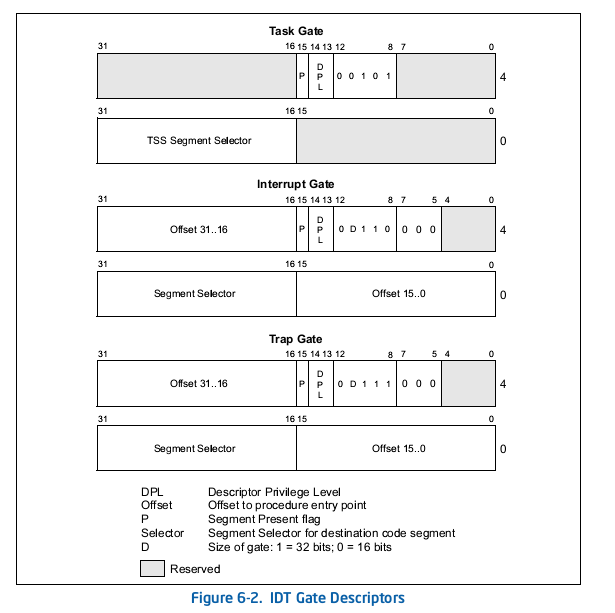
\includegraphics[width=\textwidth]{gates}
    \caption{Formato de las gates en IDT}
    \label{fig:gates}
\end{figure}



\subsubsection{Inicializar la IDT}

Para inicializar la IDT usamos una serie de macros tanto en C (para las gates) como en ASM (para las ISR) para facilitar la definición de las mismas.
De los macros generados usamos particularmente 3 de estos.
\begin{description}
\item [IDT_ENTRY_INTERRUPT] para las interrupciones de tipo 0-19, 32,33 y 40. Se setea con el descriptor de nuestro segmento flat de código de nivel 0, y offset (dividido de 0 a 15 y 16 a 31 bits por cuestiones de arquitectura) con puntero a una rutina genérica del 0-19, y específica para reloj (PIT y RTC) y teclado en interrupiones 32, 40 y 33 respectivamente. \\
Los atributos corresponden a nivel de privilegio 0, bit de present en 1 y tipo = 0xE >> 2
\item [IDT_ENTRY_DEFAULT] para las interrupciones reservadas por Intel según manual (20-31) y aquellas "libres" para el usuario que no definimos (por lo tanto, no deberían ser accedidas durante la ejecución del sistema). 
\item [IDT_ENTRY_INTERRUPT_USER] para syscalls int 0x66 con privilegios de nivel usuario para llamar a SOY, DONDE y MAPEAR.
\end{description} 

Originalmente las interrupciones no-default se encargan de imprimir por pantalla su número de interrupción con un define que se hace dentro del macro de la isr.
\begin{lstlisting} [caption={Mensaje en el macro de isr},label=macro-msg]
%macro ISR 2
global _isr%1

interrupt_msg_%1 db         %2
interrupt_msg_%1_len equ    $ \$ $ - interrupt_msg_%1

\end{lstlisting}

Todo esto quedó encapsulado en una función llamada idt_inicializar() que es ejecutada luego de cargar en IDTR un descriptor con la dirección donde se encuentra la IDT y su límite, empaquetados en el struct idt_descriptor de la cátedra.


\subsubsection{Habilitar la IDT}

\section{Ejercicio 3}

\subsection{Inicializar las páginas del kernel con identity mapping}

Para inicializar el directorio de páginas del kernel creamos una función mmu_inicializar_dir_kernel() que hace lo siguiente:

\begin{itemize}
	\item Setea en cero todos los page directory entry menos el primero, que tiene como base la dirección de su primera tabla y los bit de present y write en 1.
	\item Mapea todas las entradas dicha página con identity mapping y setea los bits de present y write en 1, logrando mapear así los primeros 4MB de memoria.
\end{itemize}

Más adelante extendimos la misma función para que mapee la página de la tarea idle, también con identity mapping.

\subsection{Activar paginación}

Para activar paginación movimos en eax el contenido de cr0, seteamos en 1 el bit de paginación (bit 31) y devolvimos a cr0 el contenido de eax.

\subsection{Ejercicio 4}

\subsubsection{Escribir rutinas para administrar el manejo de páginas}


\section{Ejercicio 5}
Como ya definimos anteriormente (\ref{rutinas}), si bien seteamos rutinas 'default' para excepciones, las rutinas de atención de interrupciones de teclado y reloj son diferentes.
Para estas interrupciones (controladas por el PIC) interactuamos con puertos I/O para luego hacer llamados a rutinas específicas ($rtc\_isr$, $keyboard\_isr$, etc) que respondan a estas interrupciones.
\\Por lo tanto lo único que haremos dentro de las $\_isr(\# int)$ definidas en $isr.asm$ será comunicar el fin de interrupción a los puertos del pic y hacer llamados a tareas correspondientes codeadas en C.
\\Caso aparte es el de la int 0x66, que es la que en la lógica del juego permitirá hacer las syscalls para llamar a $DONDE$, $SOY$ y $MAPEAR$ según un parámetro input en $eax$.

\subsection{Habilitar interrupciones de reloj}
Contamos con dos rutinas de atención a dos relojes diferentes: el RTC \footnote{Real-time clock } y el PIT \footnote{Programmable Interval Timer}, asignados a interrupciones nº 32 y 40 respectivamente. \\
Si bien en el contexto del uso dado en este sistema no presentan diferencias ambos relojes, delegamos en el RTC las cuestiones referentes al scheduler y dedicamos el PIT exlusivamente para el funcionamiento del audio \ref{audio}.
\\
\\
Para el RTC se corresponde la siguiente rutina:

\begin{lstlisting}
  void rtc_isr() {
      // Read RTC_C to ack the interruption
      outb(RTC_CMD, RTC_MASK_NMI | RTC_C);
      inb(RTC_DATA);

      game_tick();
  }
\end{lstlisting}

Donde la primer línea se encarga de reconocer la interrupción y se deshabilitan las NMI
\footnote{Non-maskable interrupt, \url{http://wiki.osdev.org/RTC\#Avoiding_NMI_and_Other_Interrupts_While_Programming}} mientras se accede el registro C del RTC (de no suceder esto, frente a determinadas interrupciones,
\href{http://wiki.osdev.org/RTC\#Interrupts_and_Register_C}{se podría deshabilitar la interrupción del RTC}). El acknowledge se completa leyendo el puerto de datos del RTC en la segunda línea. \\
Luego se hace un llamado a $game\_tick()$ (función de $game.c$) que llama a actualizarse al scheduler.



\subsection{Habilitar interrupciones de teclado}
Se lee del puerto $0x60$ un scan code que luego convertimos a ASCII usando un switch statement para cada botón de la interfaz del juego (ignorando los break codes, de modo que solo se acciona una interrupción al pulsar cada tecla).
A partir de esta conversión se determina si se actualiza la posición de un cursor, si se muestra la pantalla de restart, ayuda o se setea el debug mode \ref{isr_dbg} (entre otros).

\begin{lstlisting}
  unsigned char status2ASCII(unsigned char input){
      unsigned char output = 0;
      switch (input){
          case 0x01: // Esc
              output = 3;
              break;
          //Player 1
          case 0x11:
              output = 'W';
              break;
          case 0x12:
              output = 'E';
  // [...]
  }
\end{lstlisting}


\subsection{Debugger}
\label{isr_dbg}
Dentro de la rutina de $keyboard\_isr$, si el debugger (\ref{dbg}) se encuentra en pantalla entonces solamente se atenderá la interrupción de teclado que lo desactiva (correspondiente a la letra 'Y').
Por lo tanto no se podrán mover cursores cuando se esté mostrando.\\
Para habilitar el modo debug, se llama a la interrupción de teclado de la letra 'Y' y se habilita un flag $dbg\_enabled$ desde la función $game\_enable\_debugger$ antes de volver a la ejecución de la tarea. La próxima vez que se produzca una excepción o un error de parámetros en syscall ($game\_kill\_task$), se detendrá la ejecución y se llamará al debugger hasta que se presione nuevamente la tecla 'Y' y se salte a la tarea idle ($game\_go\_idle$) para retomar la ejecución del juego.

\subsection{Habilitar interrupción $0x66$}
Se define para la $int\ 0x66$ una syscall, cuyo funcionamiento 'ingame' detallaremos más adelante (\ref{syscalls} ).
Al entrar en la isr correspondiente se produce un llamado a funciones externas de $game.c$ en función de el parámetro pasado en $eax$, si este parámetro no es válido se procede a terminar la tarea que hizo la llamada a sistema por prevención de que esté corrupta.
\begin{lstlisting}
  global _isr0x66
  _isr0x66:
      pushad

      cmp eax, SYSCALL_DONDE
      jne .not_donde
          push ebx
          call game_donde
          add esp, 4
          jmp .end
      .not_donde:
  ;  [...]

  ; Syscall invalido
  call game_kill_task

  .end:
  popad
  iret

\end{lstlisting}

\subsection{Ejercicio 6}

\subsubsection{Definir entradas en la GDT para las TSS}

Para definir las entradas de la GDT para las TSS creamos una función gdt_setear_tss_entry que toma el offset de la gdt 
\subsection{Ejercicio 7}

\subsubsection{}



%\newpage
%\bibliography{bibliography}{}
%\bibliographystyle{plain}

\end{document}

